\section{Contact-Independent Gated van der Pauw Method}
\label{sec:gated_van_der_pauw_method}

The mobility extracted from a conventional two-terminal field-effect
transistor is obtained from the gate dependence of the terminal current. This
procedure is reliable only when the voltage drop at the source and drain
contacts is negligible compared with the voltage drop across the accumulated
channel. In organic thin-film transistors, however, the contact resistance can
be large and strongly gate dependent. It can therefore change the slope of a
transfer curve and produce an apparent mobility that is either underestimated
or, in the presence of gate-modulated injection, strongly overestimated
\cite{Bittle2016MobilityOverestimation,Natali2012ChargeInjection}.

The gated van der Pauw (gVDP) method avoids this ambiguity by combining
electrostatic charge accumulation with a four-terminal measurement of the
sheet conductance. Rolin et al. introduced the method for organic
semiconductors and demonstrated that it yields the long-range mobility of the
accumulation layer independently of the voltage losses at the current-injecting
contacts \cite{Rolin2017GVDP}. More recent work by Lee et al. showed that the
same principle corrects contact-induced mobility overestimation in short-channel
thin-film transistors and can be extended to separate channel and contact
resistances within one device \cite{Lee2024GVDPIGZO,Lee2025VoltageDrivenGVDP}.
The present thesis uses the current-driven form of the method, hereafter
denoted C-gVDP.

%%%%%%%%%%%%%%%%%%%%%%%%%%%%%%%%%%%%%%%%%%%%%%%%%%%%%%%%%%%%%%%%%%%%%%%%%%%%%%%
\subsection{Classical van der Pauw Method}

The classical van der Pauw method determines the sheet resistance of a thin
conducting film without assigning a rectangular channel length and width. Its
standard assumptions are that the film is homogeneous, approximately isotropic
in the plane, of uniform thickness, simply connected, and contacted by
sufficiently small electrodes located at its boundary. Under these conditions,
the sheet resistance is determined by the potential distribution inside the
film rather than by its external shape~\cite{VanDerPauw1958}.

\begin{figure}[htbp]
    \centering
    \scalebox{1.2}{\begin{circuitikz}[scale=0.5]
    % Insert the PDF file as a node
    \node at (0.3,0) {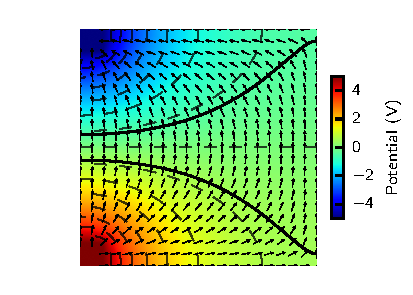
\includegraphics[width=7cm]{figures/classical-vdP.pdf}};

    \draw (-4,-4)--(-10,-4) to[current source, bipoles/length=1.5cm] (-10,4)--(-4,4);
    \node at(-10,0)[left=12pt]{$I_{34}$}; 

    \draw (4,-4)--(10,-4) to[rmeter, t = V, bipoles/length=1.5cm] (10,4)--(4,4);
    \node at(10,0)[right=12pt]{$V_{21}$}; 


    % Draw some TikZ elements
    \draw[thick, black] (-4,-4)--(4,-4)--(4,4)--(-4,4)--(-4,-4);
    \filldraw[fill = black!50, draw = black] (-5,-5)--(-3,-5)--(-3,-3)--(-5,-3)--(-5,-5);
    \filldraw[fill = black!50, draw = black] (5,-5)--(3,-5)--(3,-3)--(5,-3)--(5,-5);
    \filldraw[fill = black!50, draw = black] (-5,5)--(-3,5)--(-3,3)--(-5,3)--(-5,5);
    \filldraw[fill = black!50, draw = black] (5,5)--(3,5)--(3,3)--(5,3)--(5,5);
    \node[font=\large\bfseries] at (-4,-4) {4};
    \node[font=\large\bfseries] at (4,-4) {1};
    \node[font=\large\bfseries] at (-4,4) {3};
    \node[font=\large\bfseries] at (4,4) {2};
\end{circuitikz}}
    \caption[Classical van der Pauw measurement geometry]{Classical van der
    Pauw geometry. A current $I_{34}$ is driven between contacts 3 and 4, while
    the voltage $V_{21}$ is measured between the remaining high-impedance
    voltage probes. The dashed contours indicate equipotential lines; in
    particular, the contours passing through contacts 1 and 2 mark the two
    potentials whose difference is measured as $V_{21}$. The quiver arrows show
    the local electric-field direction and, in the Drude model, the
    corresponding current-density direction. Adapted from Ref.~\cite{Rolin2017GVDP}.}
    \label{fig:classical_vdp_geometry}
\end{figure}

For the configuration in Figure~\ref{fig:classical_vdp_geometry}, the measured
four-terminal resistance is
\begin{equation}
    R_{34,21}=\left|\frac{V_{21}}{I_{34}}\right|.
    \label{eq:vdp_four_terminal_resistance}
\end{equation}
A second independent resistance is obtained after rotating the terminals, for
example $R_{23,14}=|V_{14}/I_{23}|$. The sheet resistance $R_\mathrm{s}$ is the
solution of the van der Pauw equation~\cite{VanDerPauw1958}
\begin{equation}
    \exp\left(-\frac{\pi R_{34,21}}{R_\mathrm{s}}\right)
    +
    \exp\left(-\frac{\pi R_{23,14}}{R_\mathrm{s}}\right)
    =1.
    \label{eq:vdp_general_relation}
\end{equation}
For a fourfold-symmetric square or clover-leaf device, the complementary
resistances are ideally equal. With their averaged value $\overline{R}$, the
sheet resistance and sheet conductance reduce to
\begin{equation}
    R_\mathrm{s}=\frac{\pi}{\ln 2}\,\overline{R},
    \qquad
    \sigma_\mathrm{s}=\frac{1}{R_\mathrm{s}}
    =\frac{\ln 2}{\pi\overline{R}}.
    \label{eq:vdp_symmetric_sheet_conductance}
\end{equation}
In practice, the current direction is reversed and all four sides are measured,
which gives eight resistance values. Their average suppresses offsets caused by
small geometrical asymmetries, contact misalignment, and thermoelectric
voltages \cite{Rolin2017GVDP,Lee2024GVDPIGZO}.

The voltage probes ideally draw no current. Consequently, their metal--
semiconductor contact resistances do not produce a series voltage drop in the
measured transverse voltage. Contact resistance may still affect the voltage
required to inject the prescribed current, but it does not directly enter
Equation~\eqref{eq:vdp_symmetric_sheet_conductance}.

%%%%%%%%%%%%%%%%%%%%%%%%%%%%%%%%%%%%%%%%%%%%%%%%%%%%%%%%%%%%%%%%%%%%%%%%%%%%%%%
\subsection{Current-Driven Gated Van-der-Pauw Geometry}
\label{subsec:current_driven_gvdp}

The gated method adds a common gate electrode beneath the dielectric and the
semiconductor film. In the contact notation used in this thesis, contact 4 is
the electrical reference, a constant current $I_{34}$ is driven between
contacts 3 and 4, and contacts 1 and 2 are used only as voltage probes. The
measured probe voltages are $V_{14}$ and $V_{24}$, from which the transverse van
der Pauw voltage and the mean potential of the probed region are defined as
\begin{equation}
    V_{12}=V_{14}-V_{24},
    \qquad
    V_\mathrm{C}=\frac{V_{14}+V_{24}}{2}.
    \label{eq:gvdp_probe_voltage_and_vc}
\end{equation}
The corresponding four-terminal resistance is
\begin{equation}
    R_{34,12}=\left|\frac{V_{12}}{I_{34}}\right|.
    \label{eq:gvdp_measured_resistance}
\end{equation}
After reversing and rotating the contact configuration, the averaged resistance
$\overline{R}$ is inserted into
Equation~\eqref{eq:vdp_symmetric_sheet_conductance} to obtain the intrinsic
sheet conductance.

It is important to distinguish the two measured voltage drops. The longitudinal
voltage $V_{34}$ is the voltage that the current source must apply to establish
$I_{34}$ and therefore contains voltage losses in both the channel and the
injecting contacts. In contrast, $V_{12}$ is sensed by passive probes inside the
film and is used to determine $\sigma_\mathrm{s}$. Lee et al. refer to these as
the contact-sensitive transfer regime and the contact-independent conductance
regime, respectively \cite{Lee2025VoltageDrivenGVDP}. The current-driven method
used here employs the conductance regime for mobility extraction.

A qualitative lateral electrostatic simulation of this geometry is shown in
Appendix~\ref{app:vdp_simulation}, Figure~\ref{fig:vdp_sim_results}. The
calculation is used only to visualize how fixed contact potentials and
insulating boundaries can produce a nonuniform in-plane potential and a
corresponding nonuniform hole-density map. It is not a quantitative simulation
of the complete gated device, because the vertical gate stack is not solved
explicitly.

This qualitative picture illustrates why the internal potential
$V_\mathrm{C}$ must be included in the analysis. The gate does not act relative
to an everywhere-grounded semiconductor sheet; it acts relative to the local
semiconductor potential. Even when contact 4 is grounded, the central region of
the film acquires a finite potential under current flow. Neglecting this
potential is equivalent to assuming $V_\mathrm{C}=0$, which is justified only
in the limit of a vanishing measurement current or a negligible voltage drop
inside the film.

%%%%%%%%%%%%%%%%%%%%%%%%%%%%%%%%%%%%%%%%%%%%%%%%%%%%%%%%%%%%%%%%%%%%%%%%%%%%%%%
\subsection{Gate-Induced Sheet Density and Mobility Extraction}
\label{subsec:gvdp_density_mobility}

Within the gradual-channel and parallel-plate-capacitor approximations, the
local gate-induced sheet charge at a semiconductor potential $\phi$ is
\begin{equation}
    Q_\mathrm{2D}(\phi)
    =C_\mathrm{i}\left(V_\mathrm{G4}-\phi-V_\mathrm{T}\right),
    \label{eq:gvdp_local_sheet_charge}
\end{equation}
where $C_\mathrm{i}$ is the gate-insulator capacitance per unit area,
$V_\mathrm{G4}$ is the gate voltage relative to contact 4, and $V_\mathrm{T}$ is
the threshold voltage in the same voltage convention. Approximating the
potential of the region sampled by the voltage probes by
$\phi\simeq V_\mathrm{C}$ gives the modified two-dimensional carrier density
used in this thesis,
\begin{equation}
    \boxed{
    n_\mathrm{2D}
    =\frac{C_\mathrm{i}}{q}
    \left(V_\mathrm{G4}-V_\mathrm{C}-V_\mathrm{T}\right)
    }.
    \label{eq:gvdp_modified_carrier_density}
\end{equation}
Equation~\eqref{eq:gvdp_modified_carrier_density} is a signed carrier density.
For the $p$-type devices investigated here, the quantity in parentheses is
negative when holes are accumulated. The positive hole number density is
therefore
\begin{equation}
    p_\mathrm{2D}
    =\frac{C_\mathrm{i}}{q}
    \left|V_\mathrm{G4}-V_\mathrm{C}-V_\mathrm{T}\right|.
    \label{eq:gvdp_hole_density_magnitude}
\end{equation}

The sheet conductance is related to sheet density and mobility by
\begin{equation}
    \sigma_\mathrm{s}=q p_\mathrm{2D}\mu_\mathrm{gVDP}.
    \label{eq:gvdp_conductance_density_mobility}
\end{equation}
Combining Equations~\eqref{eq:gvdp_hole_density_magnitude} and
\eqref{eq:gvdp_conductance_density_mobility} yields
\begin{equation}
    \sigma_\mathrm{s}
    =\mu_\mathrm{gVDP}C_\mathrm{i}
    \left|V_\mathrm{G4}-V_\mathrm{C}-V_\mathrm{T}\right|.
    \label{eq:gvdp_sheet_conductance_gate_voltage}
\end{equation}
A derivation from the gradual-channel drift equation is provided in
Appendix~\ref{app:gvdp_derivation}.

If the mobility is approximately constant over the fitted high-charge-density
range, a plot of $\sigma_\mathrm{s}$ against the internal gate voltage
$V_\mathrm{G4}-V_\mathrm{C}$ is linear. The mobility follows from its slope,
\begin{equation}
    \mu_\mathrm{gVDP}
    =\frac{1}{C_\mathrm{i}}
    \left|
    \frac{\mathrm{d}\sigma_\mathrm{s}}
    {\mathrm{d}\left(V_\mathrm{G4}-V_\mathrm{C}\right)}
    \right|,
    \label{eq:gvdp_mobility_from_slope}
\end{equation}
and the horizontal intercept gives
\begin{equation}
    V_\mathrm{G4}-V_\mathrm{C}=V_\mathrm{T}.
    \label{eq:gvdp_threshold_from_intercept}
\end{equation}
The correction by $V_\mathrm{C}$ is essential. Using only
$V_\mathrm{G4}-V_\mathrm{T}$ assigns the full gate voltage to the dielectric,
even though part of it is offset by the finite potential of the conducting
sheet. This can introduce a current-dependent error in both the carrier density
and the extracted threshold voltage.

Equation~\eqref{eq:gvdp_mobility_from_slope} should not be interpreted as a
universal pointwise mobility formula when $\mu$ itself changes strongly with
carrier density. In that case, the slope contains both the mobility and its
gate-voltage dependence. The constant-mobility value is therefore extracted
only from a region in which $\sigma_\mathrm{s}$ is well described by a straight
line, as proposed by Rolin et al. \cite{Rolin2017GVDP}.

%%%%%%%%%%%%%%%%%%%%%%%%%%%%%%%%%%%%%%%%%%%%%%%%%%%%%%%%%%%%%%%%%%%%%%%%%%%%%%%
\subsection{Operating Regimes and Measurement Validity}
\label{subsec:gvdp_operating_regimes}

In a C-gVDP measurement, the source meter continuously adjusts $V_{34}$ to keep
$I_{34}$ constant while the gate voltage is swept. Close to the off-state, the
film resistance and the required injection voltage can become large. The device
then enters a saturation-like regime in which the injecting-contact potential
follows the gate voltage and the current source may approach its compliance
limit. At sufficiently strong accumulation, the required longitudinal voltage
becomes small and the probed region behaves as a linear, approximately
homogeneous conducting sheet. Rolin et al. identified these regimes through the
measured contact and probe potentials and extracted the mobility from the
high-charge-density linear regime \cite{Rolin2017GVDP}.

Reliable gVDP extraction is therefore based on the following experimental
checks:
\begin{itemize}\itemsep0em
    \item the current source remains below its voltage-compliance limit and the
    gate leakage remains negligible;
    \item $V_{12}$ scales linearly with $I_{34}$, so that the measurement is in
    the small-signal or ohmic transport regime;
    \item conductance curves measured at different current levels collapse when
    plotted against $V_\mathrm{G4}-V_\mathrm{C}$;
    \item mobility and threshold voltage are fitted only over the linear
    high-charge-density part of the conductance curve.
\end{itemize}

The use of several current levels is more than a reproducibility check. Since
$V_\mathrm{C}$ changes with the imposed current, agreement of the corrected
conductance curves demonstrates that the measured sheet conductance is a
property of the accumulated film rather than being dependent on the selected source
current. This current independence is one of the central validity criteria used
in the analysis in Chapter~4.

%%%%%%%%%%%%%%%%%%%%%%%%%%%%%%%%%%%%%%%%%%%%%%%%%%%%%%%%%%%%%%%%%%%%%%%%%%%%%%%
\subsection{Meaning and Limitations of Contact Independence}
\label{subsec:gvdp_contact_independence}

The term \emph{contact independent} refers specifically to the extraction of
the sheet voltage from non-injecting, high-impedance probes. The contact voltage
drops at the current electrodes are excluded from $V_{12}$ and therefore do not
appear directly in $R_\mathrm{s}$. This is the essential distinction from a
two-terminal OFET transfer curve, in which the measured voltage includes both
channel and contact contributions. 

The contacts are nevertheless not physically irrelevant. The injecting
electrodes must still supply the prescribed current, and poor injection can
produce large compliance voltages, nonlinear response, self-heating, or an
insufficiently accumulated region. Furthermore, the van der Pauw analysis can
be degraded by large contacts, disconnected regions, strong lateral
inhomogeneity, anisotropic transport, substantial gate leakage, or a voltage
probe with insufficient input impedance. Charge trapping and hysteresis may
also shift $V_\mathrm{T}$ between sweep directions even when the sheet
conductance itself is measured without a contact voltage drop.

Finally, $\mu_\mathrm{gVDP}$ is the macroscopic, contact-independent mobility of
carriers moving through the field-induced accumulation layer over the scale of
the thin film. It includes long-range transport barriers such as grain
boundaries, structural disorder, and trap-rich regions. It should therefore not
be identified automatically with the microscopic intragrain mobility of an
ideal crystal \cite{Rolin2017GVDP}. For the present thesis, this macroscopic
accumulation-layer mobility is the relevant quantity because it characterizes
the transport that governs actual thin-film transistor operation.
